\section*{Introduction} \thispagestyle{empty}

The aim of this fifth lab is to discover the basis of reinforcement
learning with the implementation of the Q-Learning algorithm on a rocket
stabilization problem.

It is divided in three different parts : \begin{itemize} \item Implementing
the Q-Learning algorithm \item Control the angle \item Control the hovering
\end{itemize}

\section*{Q-Learning algorithm}

The actual implementation of Q-Learning needs to be completed in the 
code skeleton. The Q-Table and every other necessary elements are
already provided.


\begin{figure}[h] \centering 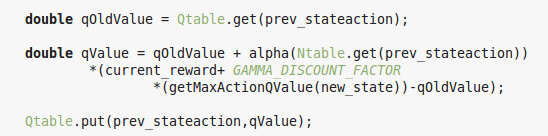
\includegraphics[width=.89\linewidth,
scale=1.5]{./images/1.png} \caption{Q-Learning formula implementation}
\end{figure} 

Basically, each iteration the Q-Table is updated with the sum of the
previous Q-Value and the product of the \textit{learning rate} and
an expression which consists in the substraction of the previous Q-value
from table to the addition of the sum of the previous reward and the
product of the discount factor multiplied by the best reward.

The \textit{learning rate} is chosen equal to 9 and the discount factor 
is 0.95, which correspond to the recommanded value(not too greedy). If the
\textit{learning rate} is high the agent learns faster. The skeleton
provides a function \textit{double alpha(int num\_tested)} which decreases 
the learning rate over time(over the multiple observations of a given
state) to achieve convergence. 

Then, the actions must be implemented. Basically an action in
this lab consists in a function of the booster states. The booster can
be turned on and off. For example the action \textit{TurnLeftForward} could
be having the right and the middle booster turned on, while the middle one
is off.  Keeping in mind that ideally we want as few different actions as
possible for the learning phase to be efficient. A good choice is to
implement \textit{forward()}, \textit{turnLeft()}, \textit{turnRight()},
and \textit{resetRockets()}, to switch off the three boosters.

\section*{Q-Learning angle controller}

The aim of this part is to control the direction of the spaceship : the
learning part is done with the angle value.

\subsection*{Defining the states}

The state are simply defined using a string wich is the result of a
concatenation between the keyword "Angle:" and the result of the angle
discretization.

Indeed to avoid an infinite number of states and therefore have an
effective Q-Learning implementation, it is necessary to discretize the
angle value. The code skeleton provides us with a discretization function.

\lstset{language=Java} 
\begin{lstlisting} 
int discretize(double value, int nrValues, double min, double max)
\end{lstlisting}

The tricky part is to find a good discretization, \textit{nrValues} should
be the smallest possible because it will correspond to the number of
states. \textit{min} and \textit{max} reduce the domains, a good choice
could be $-\Pi/4<angle<\Pi/4$ with \textit{nrValues} equal to 5. 

\subsection*{Rewards}

The angle reward function should be simple, simply returns a numerical
value.

One possible solution is to use the formula $-|angle|/\Pi$ which will
return a negative reward. 

\section*{Full Q-Learning hover controller}

Getting the spaceship to hover properly is a difficult task because it
boils down to weightening an equation of three parameters : \textit{the
angle value, the velocity on x and the velocity on y}.
A really fine tuning is necessary for a perfect result.

\subsection*{Defining the states} 

The states are defined in the same way as presviously as a string. It
is composed of the angle "A:" concatenated with its discretized value, the
velocity on y, "VY:" concatenated with its discretize value, and the same
for the velocity on Y.

The state space, \#actions multiplied by \#states is significantly bigger
than the previous one for controlling only the angle. This implies that
efficient discretizations must be implemented.

The same parameters are used to discretize the angle. To discretize the
velocities the domain is really restricted, $-1<vx,vy<1$ and only five
values are taken for each one.

In total the state space is equal to $5*5*5*4=600$.

\subsection*{Rewards}

The final reward function for hovering simply consists in the sum of the
negative rewards for velocities and the angle, each weightened by a
constant.

The tuning gives A=1.95 for the velocities and B=32*1.45 for the angle.
This results in acceptable but not perfect behaviour.

\newpage
\thispagestyle{empty}
\subsection*{Turning off exploration}

The exploration phase consists in not always picking the highest utility
action but also trying random actions with a certain probability in order
to discover all the different states.

If the exploration is turned off from the beginning, the agent still learns
from experience but does not discover every state and therefore end up in
a suboptimal policy or converge to a bad situation.

For example after 900k my agent was falling endlessly with a P\_QVAL of
-391 without being able to correct itself.
Even after reajusting the trajectory, the agent kept falling back to a poor
situation.
